\chapter{Phonons and Lattice Thermodynamics}

Atoms in a crystal are not static: they vibrate about their equilibrium sites, and those vibrations are collective, propagating through the lattice as waves. Quantized, these waves are the \emph{phonons}. This chapter builds the machinery of lattice dynamics --- the harmonic expansion of the lattice energy, the dynamical matrix, and the dispersion relation $\omega(\vect{k})$ --- and then uses it to explain two thermal properties of solids: the heat capacity (Einstein and Debye models) and the thermal conductivity (which requires anharmonic phonon--phonon scattering to exist at all).

% ============================================================
\section{From the Wave Equation to Three Dimensions}
% ============================================================

The starting point is the one-dimensional wave equation
\begin{equation}
    \pdv[2]{y}{t} = c^2 \pdv[2]{y}{x}, \qquad c = \frac{\omega}{k},
\end{equation}
whose solutions are travelling waves with phase velocity $c$. The velocity that actually transports energy is the \emph{group velocity} $\partial\omega/\partial k$, evaluated about the mean wave frequency $\omega$; a standing wave, being a superposition of counter-propagating waves, has zero group velocity.

Generalizing to three dimensions, a lattice vibration is written as
\begin{equation}
    \vect{u}(\vect{r}, t) = \tilde{\vect{u}}\,\exp\!\left(i\vect{k}\cdot\vect{r} - i\omega t\right).
\end{equation}

\begin{fact}[Rules for the dispersion relation]
\begin{enumerate}
    \item There are $3n$ different vibrational modes per unit cell, where $n$ is the number of atoms per unit cell.
    \item Each such mode has a unique frequency associated with it for a given $\vect{k}$.
    \item The amplitude of a mode is determined by the frequency of the wave and by the temperature.
\end{enumerate}
\end{fact}

% ============================================================
\section{Lattice Energy and the Harmonic Approximation}
% ============================================================

Label an atom by $j$ (its index within the unit cell) and $\ell$ (which unit cell it sits in). The total lattice energy is a sum of pair potentials,
\begin{equation}
    W = \frac{1}{2}\sum_{jj',\ell\ell'} \varphi(j\ell, j'\ell').
\end{equation}
Expanding this in a multivariate Taylor series about the equilibrium configuration and keeping the quadratic term --- the linear term vanishes at equilibrium --- gives
\begin{equation}
    W = W_0 + \frac{1}{2}\sum_{jj',\ell\ell'}\ \sum_{\alpha\beta} \Phi^{\alpha\beta}\!\begin{pmatrix} jj' \\ \ell\ell'\end{pmatrix} u_\alpha(j\ell)\, u_\beta(j'\ell'),
\end{equation}
so that the harmonic energy may be written compactly as
\begin{equation}
    E_{\text{harm}} = \frac{1}{2}\sum_{jj',\ell\ell'} \vect{u}^{T}(j\ell)\cdot \Phi \cdot \vect{u}(j'\ell')
    = \frac{1}{2}\sum_{jj',\ell\ell'}\sum_{\alpha\beta} u_\alpha(j\ell)\, \Phi_{\alpha\beta}\, u_\beta(j'\ell').
\end{equation}

\begin{definition}[Force-constant matrix]
The atomic displacement and the force-constant (Hessian) matrix are
\begin{equation}
    \vect{u}(j\ell) = \begin{bmatrix} u_x(j\ell) \\ u_y(j\ell) \\ u_z(j\ell)\end{bmatrix},
    \qquad
    \Phi_{\alpha\beta}\!\begin{pmatrix} jj' \\ \ell\ell'\end{pmatrix} = \pdv{W}{u_\alpha(j\ell)}{u_\beta(j'\ell')}.
\end{equation}
\end{definition}

Since only \emph{relative} displacements can cost energy, an equivalent form is
\begin{equation}
    E_{\text{harm}} = \frac{1}{4}\sum_{jj',\ell\ell'} \bigl[\vect{u}(j\ell) - \vect{u}(j'\ell')\bigr]^{T} \cdot \Phi\!\begin{pmatrix} jj' \\ \ell\ell'\end{pmatrix} \cdot \bigl[\vect{u}(j\ell) - \vect{u}(j'\ell')\bigr].
\end{equation}

Two assumptions underlie this whole formalism. The first is the \emph{Born--Oppenheimer approximation}: the electrons are always at equilibrium with respect to the instantaneous lattice configuration, so the ions move on a single potential energy surface. The second is that this potential is \emph{pairwise and harmonic}, as written above.

\subsection{Equation of Motion and the Dynamical Matrix}

Differentiating the harmonic energy gives the equation of motion
\begin{formula}
\begin{equation}
    m_j\, \ddot{\vect{u}}(j\ell, t) = -\sum_{j'\ell'} \Phi\!\begin{pmatrix} jj' \\ \ell\ell'\end{pmatrix} \vect{u}(j'\ell', t),
\end{equation}
\end{formula}
which is the direct analogue of the 1D spring chain $m\ddot{x}_j = K x_{j-1} + K x_{j+1} - 2K x_j$.

Because the lattice is periodic, we may use a plane-wave (travelling-wave) ansatz, exactly as Bloch's theorem does for electronic wavefunctions:
\begin{equation}
    \vect{u}(j\ell, t) = \sum_{\vect{k},\nu} \vect{U}(j, \vect{k}, \nu)\,\exp\!\left(i\vect{k}\cdot\vect{r}(j\ell) - i\omega t\right).
\end{equation}
Substituting this into the equation of motion turns the infinite set of coupled ODEs into a finite eigenvalue problem at each $\vect{k}$:
\begin{formula}[Lattice-dynamical eigenvalue problem]
\begin{equation}
    D(\vect{k})\,\vect{e}(\vect{k}, \nu) = \omega^2(\vect{k}, \nu)\, \vect{e}(\vect{k}, \nu),
    \label{eq:phon-eigen}
\end{equation}
where the polarization vector
\begin{equation}
    \vect{e} \equiv \begin{bmatrix} \vect{u}(1, \vect{k}, \nu) \\ \vect{u}(2, \vect{k}, \nu) \\ \vdots \\ \vect{u}(n, \vect{k}, \nu) \end{bmatrix}
\end{equation}
has $3n$ components and describes all of the polarization information for a given mode $\vect{k}$, for all atoms in the unit cell.
\end{formula}
Here $D(\vect{k})$ is the $3n \times 3n$ \emph{dynamical matrix}, made up of $3\times 3$ blocks that each represent the coupling between a pair of atoms (with the masses absorbed, so that the components of $\vect{e}$ are effectively $\sqrt{m_j}\,\vect{u}(j,\ell)$).

\begin{fact}[Properties of the dynamical matrix]
\begin{itemize}
    \item $D(\vect{k})$ commutes with the symmetries of the lattice.
    \item $D(\vect{k})$ is symmetric under exchange of coordinate axes, hence Hermitian.
    \item Its eigenvalue equation~\eqref{eq:phon-eigen} produces $\omega(\vect{k})$: the \emph{dispersion relation}. Since $D(\vect{k})$ is $3n \times 3n$ and Hermitian, we expect $3n$ distinct dispersion bands.
\end{itemize}
\end{fact}

If a crystal has $N$ atoms arranged in $N_\ell$ unit cells with $p$ atoms per cell, then there are $3p$ bands in total and $3pN_\ell = 3N$ unique modes. The bands separate into two families.

\begin{definition}[Acoustic and optical modes]
\emph{Acoustic} modes are the lower-frequency branches in which the atoms within a unit cell travel in the same direction; these are the modes that transmit sound. \emph{Optical} modes are the higher-frequency branches in which atoms within a cell travel in different directions, producing an oscillating dipole that interacts with light.
\end{definition}

A negative (imaginary) frequency is not merely a curiosity: it signals diverging, non-oscillatory behaviour, and hence a structural instability. Phonon calculations are therefore used to study displacive and structural phase transitions --- an unstable branch dipping below zero marks the direction in which the lattice wants to distort.

% ============================================================
\section{The One-Dimensional Chain}
% ============================================================

The simplest concrete realization is a chain of identical masses $m$ connected by springs of constant $K$ and spacing $a$ (Figure~\ref{fig:phon-chain}). Writing $\delta x_n$ for the displacement of the $n$th mass from its equilibrium site, the net force is
\begin{equation}
    F_n = K(\delta x_{n+1} - \delta x_n) + K(\delta x_{n-1} - \delta x_n) = m\, \ddot{\delta x}_n.
\end{equation}

\begin{figure}[ht]
\centering
\begin{tikzpicture}[
    spring/.style={decorate, decoration={coil, aspect=0.5, segment length=4pt, amplitude=4pt, pre length=3pt, post length=3pt}},
    mass/.style={draw, thick, fill=LightGray, minimum width=0.9cm, minimum height=0.9cm}
]
    \draw[spring] (-0.9,0) -- (0.05,0);
    \node[mass] (m0) at (0.5,0) {$m$};
    \draw[spring] (0.95,0) -- (2.55,0);
    \node[mass] (m1) at (3,0) {$m$};
    \draw[spring] (3.45,0) -- (5.05,0);
    \node[mass] (m2) at (5.5,0) {$m$};
    \draw[spring] (5.95,0) -- (6.9,0);
    % spring constants
    \node at (1.75,0.55) {$K$};
    \node at (4.25,0.55) {$K$};
    % lattice spacing
    \draw[<->] (0.5,1.1) -- (3,1.1);
    \node[above] at (1.75,1.1) {$a$};
    % displacements
    \draw[-{Latex}, ForestGreen, thick] (0.5,-0.75) -- (1.1,-0.75);
    \node[ForestGreen, below] at (0.8,-0.8) {$\delta x_0$};
    \draw[-{Latex}, ForestGreen, thick] (3,-0.75) -- (3.6,-0.75);
    \node[ForestGreen, below] at (3.3,-0.8) {$\delta x_1$};
    \draw[-{Latex}, ForestGreen, thick] (5.5,-0.75) -- (6.1,-0.75);
    \node[ForestGreen, below] at (5.8,-0.8) {$\delta x_2$};
\end{tikzpicture}
\caption{A monatomic chain of masses $m$ joined by springs of constant $K$ with lattice spacing $a$. Each mass feels a restoring force from the relative displacement of its two neighbours.}
\label{fig:phon-chain}
\end{figure}

\begin{definition}[Normal modes]
A \emph{normal mode} is a collective oscillation in which all particles move at the same frequency.
\end{definition}

Taking the normal-mode ansatz $\delta x_n = A\,e^{i\omega t - i k x_n^{\text{eq}}} = A\,e^{i\omega t - ikna}$ and substituting,
\begin{equation}
    -m\omega^2 A e^{i\omega t - ikna} = K A e^{i\omega t}\left[e^{-ik(n+1)a} + e^{-ik(n-1)a} - 2e^{-ikna}\right],
\end{equation}
so that
\begin{equation}
    m\omega^2 = 2K\bigl(1 - \cos(ka)\bigr) = 4K \sin^2\!\left(\frac{ka}{2}\right),
\end{equation}
giving

\begin{formula}[1D dispersion relation]
\begin{equation}
    \omega(k) = 2\sqrt{\frac{K}{m}}\,\left|\sin\!\left(\frac{ka}{2}\right)\right|.
    \label{eq:phon-1d-disp}
\end{equation}
\end{formula}

The dispersion is plotted in Figure~\ref{fig:phon-1d-disp}. It is periodic in $k$, so all distinct modes lie in the first Brillouin zone $-\pi/a \le k \le \pi/a$, and the maximum frequency is $2\sqrt{K/m}$ at the zone boundary.

\begin{figure}[ht]
\centering
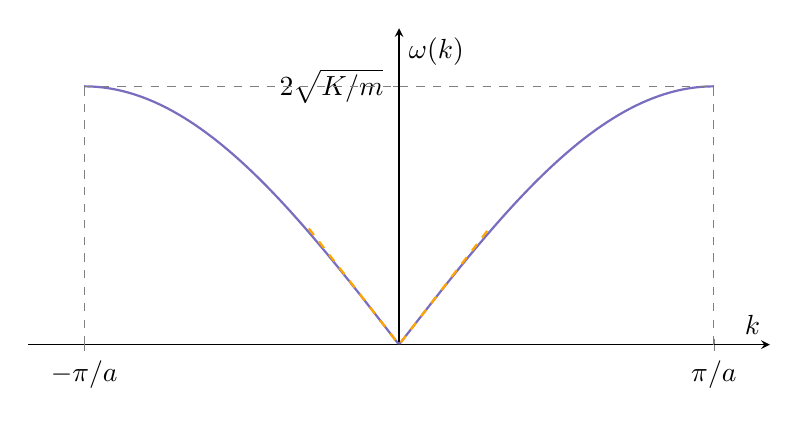
\begin{tikzpicture}
\begin{axis}[
    width=11cm, height=5.6cm,
    xlabel={$k$}, ylabel={$\omega(k)$},
    domain=-3.14159:3.14159, samples=300,
    xmin=-3.7, xmax=3.7, ymin=0, ymax=2.45,
    axis lines=middle,
    xtick={-3.14159, 0, 3.14159},
    xticklabels={$-\pi/a$, $0$, $\pi/a$},
    ytick={2}, yticklabels={$2\sqrt{K/m}$},
    every axis plot/.append style={thick},
    clip=false
]
    \addplot[Periwinkle] {2*abs(sin(deg(x/2)))};
    \addplot[Orange, dashed, domain=-0.9:0.9] {abs(x)};
    \draw[gray, dashed] (axis cs:-3.14159,0) -- (axis cs:-3.14159,2);
    \draw[gray, dashed] (axis cs:3.14159,0) -- (axis cs:3.14159,2);
    \draw[gray, dashed] (axis cs:-3.14159,2) -- (axis cs:3.14159,2);
\end{axis}
\end{tikzpicture}
\caption{Dispersion relation~\eqref{eq:phon-1d-disp} of the monatomic chain (solid), shown across the first Brillouin zone. Near $k=0$ it is linear (dashed), $\omega = v_p k$, which is the sound-wave regime; at the zone boundary the group velocity vanishes and the mode is a standing wave.}
\label{fig:phon-1d-disp}
\end{figure}

\subsection{Counting Modes}

How many modes are allowed? Exactly as many as there are atoms, $N_{\text{normal}} = N_{\text{atom}}$. To see which values of $k$ are allowed, impose periodic boundary conditions on a chain of $N$ atoms, $e^{ikNa} = 1$. Then
\begin{equation}
    \Delta k = \frac{2\pi}{Na}, \qquad \#\text{modes} = \frac{2\pi/a}{2\pi/Na} = N,
\end{equation}
confirming the count: one mode per atom, spread uniformly across the Brillouin zone.

Restricting $k$ to the first zone is not an arbitrary convention. It is the lattice analogue of the Nyquist sampling theorem: a wave sampled only at the discrete atomic sites cannot be distinguished from any longer-wavelength wave passing through the same points, so wavevectors outside the zone describe no new motion.

\subsection{The Long-Wavelength Limit}

For small $k$, expanding~\eqref{eq:phon-1d-disp},
\begin{equation}
    \omega \approx 2\sqrt{\frac{K}{m}}\cdot\frac{ka}{2} = \sqrt{\frac{K}{m}}\,ka \propto k,
\end{equation}
so the dispersion is linear with
\begin{formula}
\begin{equation}
    v_p = a\sqrt{\frac{K}{m}}, \qquad \omega = v_p k.
\end{equation}
\end{formula}
Long-wavelength lattice vibrations are therefore just sound waves travelling at a fixed speed --- the observation on which the Debye model is built.

% ============================================================
\section{Quantization and Phonon Thermodynamics}
% ============================================================

Just as we quantized electromagnetic waves into photons, we quantize each lattice normal mode into phonons:
\begin{equation}
    E = \left(n + \tfrac{1}{2}\right)\hbar\omega.
\end{equation}
Summing over all modes labelled by wavevector $\vect{k}$ and branch $\nu$,
\begin{equation}
    E(\vect{k}, \nu) = \sum_{\vect{k},\nu} \hbar\omega(\vect{k})\left(n_{\vect{k}\nu} + \tfrac{1}{2}\right).
\end{equation}

\subsection{Average Energy of a Mode}

For a single mode of frequency $\omega(\vect{k})$ at fixed $T, P, N$, the partition function is
\begin{align}
    Z &= \sum_n \exp\!\left(\frac{-\hbar\omega(\vect{k})(n + \tfrac{1}{2})}{k_B T}\right) \\
      &= \exp\!\left(\frac{-\beta\hbar\omega(\vect{k})}{2}\right)\sum_n \exp\bigl(-\beta\hbar\omega(\vect{k})\,n\bigr)
       = \frac{\exp\!\left(-\beta\hbar\omega(\vect{k})/2\right)}{1 - \exp\bigl(-\beta\hbar\omega(\vect{k})\bigr)},
\end{align}
a geometric series. The average energy follows from $\langle U_{\vect{k}}\rangle = -\partial_\beta \ln Z$:

\begin{formula}[Average energy of a mode]
\begin{equation}
    \langle U_{\vect{k}}\rangle = \hbar\omega(\vect{k})\left[\langle n_{\vect{k}}\rangle + \tfrac{1}{2}\right],
    \qquad
    \langle n_{\vect{k}}\rangle \equiv \frac{1}{\exp\!\left(\dfrac{\hbar\omega(\vect{k})}{k_B T}\right) - 1},
\end{equation}
where $\langle n_{\vect{k}}\rangle$ --- the Planck (Bose--Einstein) distribution --- is the average occupation of a given $\vect{k}$-mode at temperature $T$.
\end{formula}

Each excitation mode is a boson of frequency $\omega(\vect{k})$ and is occupied $n_B(\beta\hbar\omega(\vect{k}))$ times on average. The physical content of the distribution is that higher-frequency (higher-energy) modes are exponentially suppressed and hence much less occupied, as Figure~\ref{fig:phon-bose} shows.

\begin{figure}[ht]
\centering
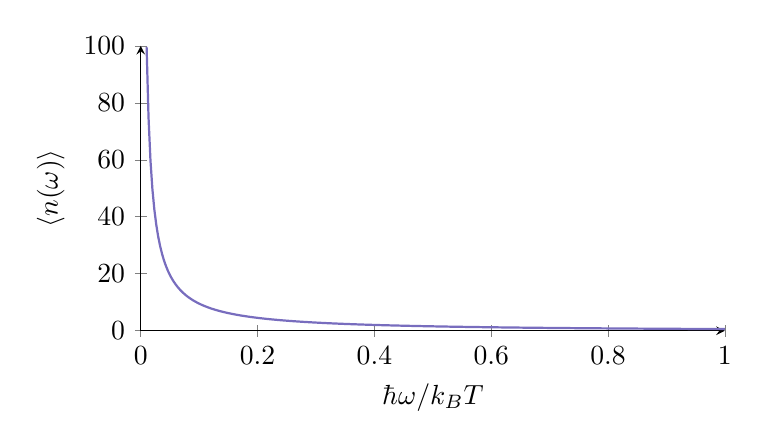
\begin{tikzpicture}
\begin{axis}[
    width=9cm, height=5.2cm,
    xlabel={$\hbar\omega / k_B T$}, ylabel={$\langle n(\omega)\rangle$},
    domain=0.01:1.0, samples=300,
    xmin=0, xmax=1.0, ymin=0, ymax=100,
    axis lines=left,
    every axis plot/.append style={thick},
]
    \addplot[Periwinkle] {1/(exp(x) - 1)};
\end{axis}
\end{tikzpicture}
\caption{The Planck distribution $\langle n(\omega)\rangle = [\exp(\hbar\omega/k_B T) - 1]^{-1}$, which fixes the occupancy of a mode of frequency $\omega$ in thermal equilibrium. Low-frequency modes are heavily occupied; high-frequency modes are exponentially frozen out.}
\label{fig:phon-bose}
\end{figure}

\subsection{Internal Energy, Heat Capacity, and the Density of States}

Summing the contributions from all phonon modes,
\begin{equation}
    \langle U \rangle = \sum_{\vect{k},\nu} \hbar\omega(\vect{k},\nu)\left[\langle n_{\vect{k}}\rangle + \tfrac{1}{2}\right].
\end{equation}
For small $\Delta k$ the sum becomes an integral over frequency weighted by the number of modes at each frequency:

\begin{formula}[Phonon internal energy and heat capacity]
\begin{equation}
    \langle U \rangle \approx \int_0^\infty \dd\omega\, g(\omega)\, \hbar\omega\left(\langle n(\omega)\rangle + \tfrac{1}{2}\right),
    \qquad
    C_V = \left.\pdv{U}{T}\right|_V = \int_0^\infty \dd\omega\, g(\omega)\,\hbar\omega\,\pdv{\langle n(\omega)\rangle}{T}.
\end{equation}
\end{formula}

\begin{definition}[Density of states]
The phonon density of states counts how many unique modes exist at a given frequency:
\begin{equation}
    g(\omega) \equiv \frac{V}{8\pi^3}\sum_{s=1}^{3p} \int_{\text{BZ}} \dd\vect{k}\;\delta\bigl(\omega - \omega(\vect{k},s)\bigr).
    \label{eq:phon-dos}
\end{equation}
\end{definition}

% ============================================================
\section{The Einstein and Debye Models}
% ============================================================

\subsection{Einstein Approach}

The Einstein model takes $\omega(\vect{k}) = \omega_E$ constant, so that $g(\omega)$ is a delta function at $\omega_E$ and every mode is an independent oscillator of the same frequency. In the high-$T$ limit this reproduces the classical Dulong--Petit result, $C_V = 3Nk_B$. In the low-$T$ limit, however, it predicts an exponential suppression $C_V \propto \exp(-\hbar\omega_E/k_B T)$, whereas experiment shows that most materials have $C_V \propto T^3$ at low temperature. This discrepancy is what Debye set out to fix.

\subsection{Debye Approach}

Debye's insight was that the oscillation of atoms in a solid is the same thing as sound. He therefore kept only the acoustic modes and used the long-wavelength dispersion
\begin{equation}
    \omega(k) = c\,k, \qquad k \equiv |\vect{k}|.
\end{equation}
For each wavevector $\vect{k}$ there are three kinds of mode --- one longitudinal and two transverse (Figure~\ref{fig:phon-polarizations}) --- and all three are assumed to travel at the same velocity.

\begin{figure}[ht]
\centering
\begin{tikzpicture}[scale=1.0]
    % Longitudinal
    \node at (1.9,1.3) {Longitudinal};
    \foreach \x in {0, 1.1, 1.5, 1.9, 2.3, 3.1, 3.9} {
        \fill[Periwinkle] (\x,0) circle (0.12);
    }
    \draw[thick] (0.12,0) -- (0.98,0);
    \draw[thick] (2.42,0) -- (2.98,0);
    \draw[thick] (3.22,0) -- (3.78,0);
    \foreach \x in {1.1, 1.5, 1.9, 2.3} {
        \draw[-{Latex}, Orange, thick] (\x,0.28) -- ++(0.35,0);
    }
    % Transverse 1 (vertical)
    \begin{scope}[xshift=5.2cm]
        \node at (1.6,1.3) {Transverse 1};
        \draw[thick, Periwinkle, decorate, decoration={snake, amplitude=4pt, segment length=10pt}] (0,0) -- (3.2,0);
        \draw[-{Latex}, thick] (1.6,-0.75) -- (1.6,0.85);
    \end{scope}
    % Transverse 2 (out of plane, drawn tilted)
    \begin{scope}[xshift=9.4cm]
        \node at (1.6,1.3) {Transverse 2};
        \draw[thick, Periwinkle, decorate, decoration={snake, amplitude=4pt, segment length=10pt}] (0,0) -- (3.2,0);
        \draw[-{Latex}, thick] (1.2,-0.6) -- (2.0,0.85);
    \end{scope}
\end{tikzpicture}
\caption{The three acoustic polarizations for a given $\vect{k}$: one longitudinal mode, in which displacements are along the propagation direction, and two mutually perpendicular transverse modes. Debye assumes all three have the same velocity.}
\label{fig:phon-polarizations}
\end{figure}

Imposing periodic (``von K\'arm\'an'') boundary conditions on a hypertorus of side $L$ gives
\begin{equation}
    \vect{k} = \frac{2\pi}{L}(n_1, n_2, n_3),
\end{equation}
so each $\vect{k}$-point occupies a volume $(2\pi/L)^3$ in reciprocal space, and sums over modes become integrals:
\begin{equation}
    \sum_{\vect{k}} \approx \frac{L^3}{(2\pi)^3}\int \dd\vect{k}.
\end{equation}
Counting states inside a sphere of radius $k$,
\begin{equation}
    \phi(k) = \frac{4}{3}\pi k^3 \cdot \frac{V}{8\pi^3} = \frac{V}{6\pi^2}k^3
    \quad\Longrightarrow\quad
    g(k) = \dv{\phi}{k} = \frac{V}{2\pi^2}k^2.
\end{equation}
Equivalently, evaluating the definition~\eqref{eq:phon-dos} with $\omega = ck$,
\begin{equation}
    g(\omega) = \frac{V}{8\pi^3}\sum_{s=1}^{3p}\int_{\text{BZ}} 4\pi k^2\,\dd k\,\delta(\omega - ck)
    = \frac{V}{8\pi^3}\,4\pi\!\left(\frac{\omega}{c}\right)^{2}\frac{1}{c}\sum_{s=1}^{3p}\int_{\text{BZ}}\dd k .
\end{equation}

To find the expected energy we sum over all $\vect{k}$-modes and polarizations,
\begin{equation}
    \langle E\rangle = 3\sum_{\vect{k}} \hbar\omega(\vect{k})\left[n_B\bigl(\beta\hbar\omega(\vect{k})\bigr) + \tfrac{1}{2}\right]
    = 3\,\frac{L^3}{(2\pi)^3}\int \dd\vect{k}\; \hbar\omega(\vect{k})\left(n_B + \tfrac{1}{2}\right),
\end{equation}
and by spherical symmetry $\int \dd\vect{k} = 4\pi\int_0^\infty k^2\,\dd k$, so
\begin{equation}
    \langle E\rangle = 3\,\frac{4\pi L^3}{(2\pi)^3}\int_0^\omega \omega^2\,\dd\omega \left(\frac{1}{v^3}\right)(\hbar\omega)\left[n_B(\beta\hbar\omega) + \tfrac{1}{2}\right].
\end{equation}
Letting $n = N/L^3$ be the atomic concentration, we read off the Debye density of states:

\begin{formula}[Debye density of states and frequency]
\begin{equation}
    g(\omega) = N\left[\frac{12\pi\omega^2}{(2\pi)^3 n v^3}\right] = \frac{9N\omega^2}{\omega_D^3},
    \qquad \omega_D^3 = 6\pi^2 n v^3,
\end{equation}
where $g(\omega)$ represents the number of oscillation modes between frequencies $\omega$ and $\omega + \dd\omega$.
\end{formula}

Then
\begin{equation}
    \langle E\rangle = \int_0^\infty \dd\omega\; \underbrace{g(\omega)}_{\#\text{ of modes}}\;\underbrace{(\hbar\omega)\left[n_B(\beta\hbar\omega) + \tfrac{1}{2}\right]}_{\text{expected energy per mode}},
\end{equation}
where the $\tfrac{1}{2}$ contributes only a temperature-independent zero-point energy.

\subsection{The \texorpdfstring{$T^3$}{T\textasciicircum 3} Law}

Substituting $x \equiv \beta\hbar\omega$ and dropping the zero-point constant,
\begin{equation}
    \langle E\rangle = \frac{9N\hbar}{\omega_D^3 (\beta\hbar)^4}\int_0^\infty \dd x\,\frac{x^3}{e^x - 1} + \text{($T$-independent constant)}.
\end{equation}
The integral is a Riemann-zeta integral equal to $\pi^4/15$, so
\begin{equation}
    \langle E\rangle = 9N \frac{(k_B T)^4}{(\hbar\omega_D)^3}\frac{\pi^4}{15} + \text{const},
\end{equation}
and therefore
\begin{equation}
    C_V = \pdv{\langle E\rangle}{T} = N k_B \frac{(k_B T)^3}{(\hbar\omega_D)^3}\frac{12\pi^4}{5} \sim T^3.
\end{equation}

\begin{formula}[Debye heat capacity at low $T$]
Writing $k_B \theta_D = \hbar\omega_D$,
\begin{equation}
    C_V = N k_B \frac{T^3}{\theta_D^3}\frac{12\pi^4}{5}, \qquad \theta_D \equiv \frac{\hbar\omega_D}{k_B}.
\end{equation}
\end{formula}

\begin{definition}[Debye temperature]
$\theta_D = \hbar\omega_D/k_B$ is the temperature scale marking the transition from classical (Dulong--Petit) to quantum behaviour --- the phonon analogue of the Fermi temperature $T_F$.
\end{definition}

\subsection{The Cutoff Frequency}

There is a problem with the calculation as it stands: $C_V$ must converge to $3Nk_B$ in the high-$T$ limit, but an unrestricted $\omega$ integral does not. The fix is to only consider frequencies up to a cutoff such that the total number of normal modes equals the number of degrees of freedom of the system:
\begin{equation}
    3N = \int_0^{\omega_{\text{cutoff}}} \dd\omega\, g(\omega).
\end{equation}
At low $T$ the cutoff does not matter, because $n_B \to 0$ very quickly. At high $T$, on the other hand,
\begin{equation}
    n_B = \frac{1}{e^{\beta\hbar\omega} - 1} \approx \frac{1}{\beta\hbar\omega} = \frac{k_B T}{\hbar\omega},
\end{equation}
so
\begin{equation}
    \langle E\rangle = \int_0^{\omega_{\text{cutoff}}} \dd\omega\, g(\omega)\,\hbar\omega\cdot\frac{k_B T}{\hbar\omega} = 3Nk_B T,
\end{equation}
as expected. Evaluating the mode-counting condition with the Debye density of states,
\begin{equation}
    3N = \int_0^{\omega_{\text{cutoff}}}\dd\omega\, g(\omega) = 9N\int_0^{\omega_{\text{cut}}}\dd\omega\,\frac{\omega^2}{\omega_D^3} = 3N\frac{\omega_{\text{cut}}^3}{\omega_D^3},
\end{equation}
so that
\begin{formula}
\begin{equation}
    \omega_{\text{cutoff}} = \omega_{\text{Debye}}.
\end{equation}
\end{formula}
The Debye frequency is thus the maximum possible phonon frequency of the lattice, and it is fixed self-consistently rather than being an extra parameter. Figure~\ref{fig:phon-cv} compares the Debye and Einstein heat capacities.

\begin{figure}[ht]
\centering
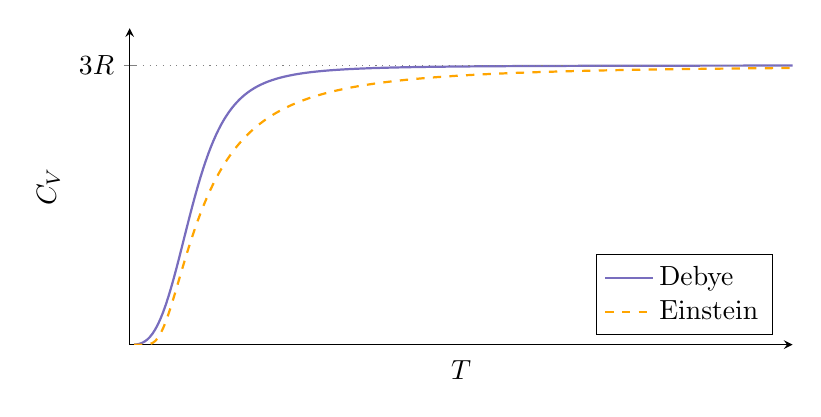
\begin{tikzpicture}
\begin{axis}[
    width=10cm, height=5.6cm,
    xlabel={$T$}, ylabel={$C_V$},
    domain=0.02:3, samples=250,
    xmin=0, xmax=3, ymin=0, ymax=3.4,
    axis lines=left,
    xtick=\empty, ytick={3}, yticklabels={$3R$},
    legend pos=south east, legend cell align=left,
    every axis plot/.append style={thick},
]
    \addplot[Periwinkle] {3*(1 - exp(-(x^3)/(0.09 + x^3)*3.2))/(1 - exp(-3.2))};
    \addlegendentry{Debye}
    \addplot[Orange, dashed] {3*(1/x)^2*exp(1/x)/((exp(1/x)-1)^2)};
    \addlegendentry{Einstein}
    \draw[gray, dotted] (axis cs:0,3) -- (axis cs:3,3);
\end{axis}
\end{tikzpicture}
\caption{Debye and Einstein specific heats. Both saturate at the classical Dulong--Petit value $3R$ at high temperature, but at low temperature the Debye model gives $C_V \propto T^3$ while the Einstein model falls off exponentially fast.}
\label{fig:phon-cv}
\end{figure}

\begin{fact}[Shortcomings of Debye theory]
\begin{itemize}
    \item The cutoff is introduced somewhat ad hoc.
    \item The dispersion $\omega = vk$ only applies at large wavelength / low $k$; at high enough $k$ the linear relation no longer holds.
    \item Metals have an additional linear electronic term, $C = \gamma T + \alpha T^3$.
\end{itemize}
\end{fact}

% ============================================================
\section{Thermal Conductivity}
% ============================================================

Heat flow is described by Fourier's law
\begin{equation}
    \vect{j}_u = -\kappa \grad T, \qquad [j] = \frac{\text{energy transmitted}}{\text{unit area}\cdot\text{unit time}},
\end{equation}
and the kinetic-theory expression for the thermal conductivity of a gas is
\begin{equation}
    \kappa = \tfrac{1}{3} C \langle v\rangle \ell,
\end{equation}
with $C$ the heat capacity, $\langle v\rangle$ the average velocity, and $\ell$ the mean free path.

\subsection{Heuristic Derivation}

If a particle moves from a region at $T$ to one at $T + \Delta T$ it gains energy $C\,\Delta T$. Writing
\begin{equation}
    \Delta T = \pdv{T}{x}\,\dd x = \pdv{T}{x}\langle v_x\rangle \tau,
\end{equation}
with $\tau$ the average time between collisions, the energy gain per particle is $\Delta U = C\langle v_x\rangle \tau\, \partial T/\partial x$, and the total flux is
\begin{equation}
    j = n\,\Delta U \cdot \langle v_x \rangle = n C \langle v_x\rangle^2 \tau \pdv{T}{x}
    \quad\Longrightarrow\quad
    j_u = -\tfrac{1}{3}C_V \langle v_x\rangle \ell \pdv{T}{x}.
\end{equation}

The same argument runs through in the phonon language. Consider two regions at $T$ and $T + \Delta T$ separated by a mean free path $\lambda$, assuming an isotropic crystal, a constant group velocity $v$, and a mean free path $\lambda = v\tau$. Then $\Delta T = \lambda\,\partial T/\partial x = v\tau\,\partial T/\partial x$, and the change in occupation is
\begin{equation}
    n(T + \Delta T) - n(T) = \Delta T \pdv{n}{T} = v\tau \pdv{T}{x}\pdv{n}{T}.
\end{equation}
The heat current is then
\begin{align}
    J &= -v\,\Delta U_{\text{ph}} = -v\int \dd\omega\, g(\omega)\,\hbar\omega\,\bigl(n_{T + \Delta T}(\omega) - n_T(\omega)\bigr) \\
      &= -v\int \dd\omega\, g(\omega)\,\hbar\omega\,\pdv{n}{T}\cdot v\tau \pdv{T}{x}
       = -\tfrac{1}{3}\langle v\rangle^2 \tau\, C_V \pdv{T}{x},
\end{align}
where the bracketed integral is recognised as $C_V$. Hence

\begin{formula}[Phonon thermal conductivity]
\begin{equation}
    \kappa = \tfrac{1}{3}\langle v^2\rangle\, \tau\, C_V .
    \label{eq:phon-kappa}
\end{equation}
\end{formula}

More formally, the phonon heat flux is
\begin{equation}
    \vect{j} = \frac{1}{(2\pi)^3}\int \hbar\omega\, \vect{v}_g\, n_{\vect{k}}\, \dd^3\vect{k}.
\end{equation}

\subsection{Why Phonons Scatter}

The mean free path $\ell$ is determined by geometrical scattering and by phonon--phonon-like scattering. This is where the harmonic approximation fails outright: in a purely harmonic crystal the plane waves are exact eigenstates, phonons do not interact with each other, and there is no mechanism to redistribute energy or momentum --- so there is no thermal resistivity at all. Yet the distribution of phonons \emph{must} change over time to reach thermal equilibrium at the local temperatures $T_1, T_2$ set by the temperature gradient.

Two candidate mechanisms fail on their own. Single-phonon scattering off a static imperfection or a crystal boundary cannot change the distribution, because $\omega_{\text{in}} = \omega_{\text{out}}$. And a three-phonon process with $\vect{k}_1 + \vect{k}_2 = \vect{k}_3$ conserves the total wavevector exactly; if the sum of reduced wavevectors is conserved, the average $\langle \vect{k}\rangle$ is fixed by the Bose--Einstein distribution
\begin{equation}
    n_{\vect{k}} = \left[\exp\!\left(\frac{\hbar\omega(\vect{k}) - \vect{v}\cdot\vect{k}}{k_B T}\right) - 1\right]^{-1},
\end{equation}
which describes a drifting phonon gas that never relaxes. The fix is to add anharmonic terms to $V_{\text{harm}}$: plane waves are then no longer exact solutions, and phonons must eventually decay or scatter into other phonons.

\begin{definition}[Umklapp process]
An \emph{Umklapp} (U) process is a three-phonon process in which momentum is conserved only up to a reciprocal lattice vector $\vect{g}$:
\begin{equation}
    \vect{k}_1 + \vect{k}_2 = \vect{k}_3 + \vect{g}.
\end{equation}
\end{definition}

Figure~\ref{fig:phon-scattering} contrasts the three relevant scattering channels: normal (N) processes, which conserve momentum and energy; Umklapp (U) processes, which do not; and boundary (B) or defect (D) scattering, which conserves energy only. Because different mechanisms dominate in different temperature regimes, the scattering rates add:
\begin{formula}[Matthiessen-type rule for phonons]
\begin{equation}
    \frac{1}{\tau} = \frac{1}{\tau_U} + \frac{1}{\tau_D} + \frac{1}{\tau_B}.
\end{equation}
\end{formula}

\begin{figure}[ht]
\centering
\begin{tikzpicture}[scale=1.0, every node/.style={font=\small}]
    % --- Normal scattering ---
    \begin{scope}
        \node[above] at (1.4,2.9) {Normal (N)};
        \draw[fill=LightGray!40] (0,0) rectangle (2.8,2.6);
        \node[anchor=north west, font=\scriptsize] at (0.05,2.58) {BZ};
        \coordinate (o) at (1.3,0.9);
        \draw[-{Latex}, thick] (o) -- ++(-0.5,1.3) node[above] {$\vect{k}$};
        \draw[-{Latex}, thick] (o) -- ++(0.7,-0.6) node[below] {$\vect{k}'$};
        \draw[-{Latex}, thick, Periwinkle] (o) -- ++(0.9,0.6) node[right] {$\vect{k}+\vect{k}'$};
    \end{scope}
    % --- Umklapp scattering ---
    \begin{scope}[xshift=4.6cm]
        \node[above] at (1.4,2.9) {Umklapp (U)};
        \draw[fill=LightGray!40] (0,0) rectangle (2.8,2.6);
        \node[anchor=north west, font=\scriptsize] at (0.05,2.58) {BZ};
        \coordinate (o2) at (1.5,1.2);
        \draw[-{Latex}, thick] (o2) -- ++(0.7,1.1) node[above] {$\vect{k}'$};
        \draw[-{Latex}, thick] (o2) -- ++(0.6,-0.9) node[below] {$\vect{k}$};
        \draw[-{Latex}, thick, Periwinkle] (o2) -- ++(-1.2,0) node[left] {$\vect{k}+\vect{k}'+\vect{g}$};
        \draw[-{Latex}, thick, Orange, dashed] (o2) ++(0.05,-0.22) -- ++(1.3,0) node[right] {$\vect{g}$};
    \end{scope}
    % --- Boundary / defect scattering ---
    \begin{scope}[xshift=9.6cm]
        \node[above] at (1.4,2.9) {Boundary / defect};
        \draw[fill=LightGray!40] (0.15,0.15) -- (1.1,0) -- (2.5,0.6) -- (2.5,2.1) -- (1.3,2.6) -- (0,1.7) -- cycle;
        \draw[-{Latex}, thick] (0.5,0.6) -- (1.1,2.1);
        \draw[-{Latex}, thick] (1.15,2.2) -- (1.6,0.5);
        \draw[-{Latex}, thick] (1.65,0.45) -- (2.35,1.9);
        \fill[Orange] (1.12,2.15) circle (1.6pt);
        \fill[Orange] (1.62,0.47) circle (1.6pt);
    \end{scope}
\end{tikzpicture}
\caption{Three phonon scattering channels drawn in the Brillouin zone. Normal processes conserve both momentum and energy; Umklapp processes conserve momentum only up to a reciprocal lattice vector $\vect{g}$, and so degrade the heat current; boundary and defect scattering conserve energy but randomize direction.}
\label{fig:phon-scattering}
\end{figure}

The full description of how the phonon distribution evolves under a temperature gradient is the Peierls--Boltzmann transport equation,
\begin{formula}[Peierls--Boltzmann transport equation]
\begin{equation}
    \underbrace{\vect{v}(\vect{k},\nu)}_{\text{phonon velocity}}\cdot\underbrace{\grad T}_{\text{temp.\ gradient}}\underbrace{\left(\pdv{n(\vect{k},\nu)}{T}\right)}_{\text{change in boson dist.}} = \underbrace{\left(\pdv{n(\vect{k},\nu)}{t}\right)_{\text{scatter}}}_{\text{time evolution of dist.}},
\end{equation}
\end{formula}
whose solution yields the relaxation time $\tau(\vect{k},\nu)$ entering~\eqref{eq:phon-kappa}.

% ============================================================
\section{Temperature Regimes of the Thermal Conductivity}
% ============================================================

With $\kappa = \tfrac{1}{3}\langle v^2\rangle C_V \tau$ in hand, the temperature dependence of $\kappa$ follows from whichever of $C_V$ and $\tau$ varies most strongly.

\subsection{Low Temperature: \texorpdfstring{$T \ll \theta_D$}{T much less than theta D}}

Umklapp scattering is suppressed, because almost no phonons have large enough wavevectors. Surface scattering sets $\tau$, and the mean free path is limited by the length scale $L$ of the boundaries:
\begin{equation}
    \tau \approx \tau_B = \frac{L}{\langle v\rangle},
\end{equation}
which is constant. Therefore the heat capacity alone sets the temperature trend:
\begin{formula}
\begin{equation}
    \kappa(T \ll \theta_D) \propto T^3,
\end{equation}
\end{formula}
since $C_V \sim T^3$ and $\ell$ is constant.

\subsection{High Temperature: \texorpdfstring{$T > 0.5\,\theta_D$}{T above half theta D}}

Here $C_V$ is close to the Dulong--Petit limit, so it is roughly constant. A non-negligible fraction of all modes takes part in scattering, and Umklapp dominates. Since
\begin{equation}
    \langle n(\omega)\rangle \approx \frac{k_B T}{\hbar\omega} \propto T,
    \qquad
    \tau \approx \tau_U \propto \frac{1}{\langle n(\omega)\rangle} = \frac{1}{T},
\end{equation}
we obtain
\begin{formula}
\begin{equation}
    \kappa(T > 0.5\,\theta_D) \propto \frac{1}{T}.
\end{equation}
\end{formula}

\subsection{Intermediate Temperature: \texorpdfstring{$0.1\,\theta_D \lesssim T \lesssim 0.5\,\theta_D$}{0.1 to 0.5 theta D}}

In between, defect and Umklapp scattering compete. For Umklapp scattering to occur at all, one needs a very pure sample (so that defect scattering is weak), and at least one of the interacting phonons in a three-phonon process must have a wavevector at least half the ``radius'' of the Brillouin zone. Approximating that radius by
\begin{equation}
    k_D \equiv \frac{\omega_D}{v},
\end{equation}
the occupation of the relevant modes is activated,
\begin{equation}
    \langle n(\omega = \omega_D/2)\rangle \approx \exp\!\left(-\frac{\theta_D}{2T}\right),
    \qquad
    \tau_U \sim \frac{1}{\langle n\rangle} \propto \exp\!\left(\frac{\theta_D}{2T}\right),
\end{equation}
so that
\begin{formula}
\begin{equation}
    \kappa \propto \exp\!\left(\frac{\theta_D}{2T}\right).
\end{equation}
\end{formula}
Reality is more complicated: defect (Rayleigh) scattering, with $\tau_D^{-1} \sim \omega^4$, mostly dominates, but Umklapp scattering is also present, and the competition between the two is what the Debye--Callaway model (1959) describes. The resulting $\kappa(T)$ has the characteristic peaked shape of Figure~\ref{fig:phon-kappa}, seen experimentally in diamond ($\theta_D \approx 1880$~K) and germanium ($\theta_D \approx 370$~K).

\begin{figure}[ht]
\centering
\begin{tikzpicture}
\begin{axis}[
    width=10cm, height=6cm,
    xlabel={$T$}, ylabel={$\kappa$},
    xmode=log, ymode=log,
    domain=1:400, samples=200,
    xmin=1, xmax=400, ymin=0.5, ymax=400,
    axis lines=left,
    xtick=\empty, ytick=\empty,
    every axis plot/.append style={thick},
    clip=false
]
    \addplot[Periwinkle] {1/( 1/(0.9*x^3) + 1/(300*exp(20/x)) + x/25 )};
    \node[Orange, anchor=west] at (axis cs:1.3,20) {$\propto T^3$};
    \node[Orange, anchor=west] at (axis cs:11,220) {$\propto \exp(\theta_D/2T)$};
    \node[Orange, anchor=west] at (axis cs:150,25) {$\propto 1/T$};
\end{axis}
\end{tikzpicture}
\caption{Schematic phonon thermal conductivity of a good insulating crystal on log--log axes. Boundary scattering gives $\kappa \propto T^3$ at low $T$; Umklapp activation gives the exponential rise and the peak at intermediate $T$; frequent Umklapp scattering gives $\kappa \propto 1/T$ at high $T$.}
\label{fig:phon-kappa}
\end{figure}

% ============================================================
\section{Modern Lattice Thermodynamics}
% ============================================================

Two computational tasks make up the modern practice of the subject. The first is the determination of the coupling constants
\begin{equation}
    \Phi_{\alpha\beta}(j\ell; j'\ell') = \pdv{V}{u_\alpha(j\ell)}{u_\beta(j'\ell')},
\end{equation}
obtained from DFT or molecular dynamics calculations of the potential $V$, with space-group symmetry used to reduce the number of independent constants. The second is the determination of the thermal conductivity, by solving the Peierls--Boltzmann transport equation for $\tau(\vect{k},\nu)$.

An application is the search for thermoelectric \emph{phonon glasses}: materials that conduct electricity like a metal but conduct heat like a glass, maximizing the figure of merit
\begin{equation}
    \mathrm{ZT} = S^2 \frac{\sigma T}{\kappa}.
\end{equation}
Such materials show distinctly non-Debye--Callaway behaviour in $\kappa(T)$.

\begin{fact}[Summary]
\begin{enumerate}
    \item \emph{Lattice dynamics} provides a rigorous foundation for quantifying phonon modes via their dispersion, amplitude vectors, and density of states.
    \item \emph{The Debye model} treats phonons as quantized harmonic oscillators whose thermodynamics gives the heat capacity, and in particular the $T^3$ law at low temperature.
    \item \emph{The Debye--Callaway model} includes anharmonic phonon interactions (phonon--phonon, defect, boundary), which are what explain the thermal conductivity of materials in the different temperature regimes.
\end{enumerate}
\end{fact}
